Tools are necessary to test concurrency, the standard approach does not suffice.
In this chapter we present and evaluate \dejafu{}, our library for testing
concurrency in Haskell.  We discuss the scope of the tool~\sref{dejafu-scope}
and present our abstraction over the GHC Haskell concurrency
functionality~\sref{dejafu-monadconc}.  We explain how programs using our
abstraction are executed~\sref{dejafu-execution} and
tested~\sref{dejafu-testing}, and argue the correctness of the testing
approach~\sref{dejafu-correctness}.  We present three case
studies~\sref{dejafu-casestudies}, evaluate the usefulness of \dejafu{} for
testing pre-existing code~\sref{dejafu-evaluation}, and finally draw conclusions
and present further work~\sref{dejafu-conclusions}.

This chapter is derived from our previous work \cite{walker2015} and
\cite{YCS-2016-503}.

\todo{Note: discussion of random scheduling is in chapter 6 (swarm) and chapter 9 (eval \& conclusions), so just have brief forward refs in this chapter}

\section{Scope}
\label{sec:dejafu-scope}

We aim to support most of the functionality of GHC’s concurrency API, as made
available through the Control.Concurrent and Control.Exception module
hierarchies, which does not unavoidably require support from the runtime system.

In particular, we do not support:

\begin{itemize}
\item Blocking a thread until a file descriptor becomes available, as this
  introduces an additional source of nondeterminism.
\item Throwing an exception to a thread if it becomes deadlocked, as we cannot
  reliably detect deadlock involving only a subset of threads without support
  from the garbage collector.
\item Querying which capability (OS thread) a Haskell thread is running on, as
  this introduces an additional source of nondeterminism.
\end{itemize}

We also do not yet support \emph{bound threads}: a Haskell thread which will
always run on the same, unique, OS thread.  Bound threads are essential for
using the FFI to call libraries which use thread-local state, to ensure the
Haskell thread always sees its state and never the state of another thread.  We
have a prototype implementation, which is not yet present in a released version
of \dejafu{}\footnote{\url{https://github.com/barrucadu/dejafu/issues/126}}.

\section{Abstracting over \texttt{IO}}
\label{sec:dejafu-monadconc}

Recall from \secref{sct-fundamentals} that there are three ways of implementing
a concurrency testing tool:

\begin{itemize}
\item Override the concurrency primitives of the programming language.
\item Instrument the source program.
\item Instrument the compiled program.
\end{itemize}

We adopt the first approach in \dejafu{}.  Haskell's typeclass machinery lets us
specify an interface for concurrency, and to provide different concrete
implementations.  There is one implementation using the \verb|IO| type and the
standard functions; there is another using our own type, based on continuations
which we can inspect.

\begin{figure}[t]
  \centering
  \begin{lstlisting}
class (Monad m, {- other constraints omitted -}) => MonadConc m where
  type MVar m :: * -> *
  -- other types omitted

  newEmptyMVar :: m (MVar m a)
  newEmptyMVar = newEmptyMVarN ""

  newEmptyMVarN :: String -> m (MVar m a)
  newEmptyMVarN _ = newEmptyMVar

  putMVar  :: MVar m a -> a -> m ()
  readMVar :: MVar m a -> m a
  takeMVar :: MVar m a -> m a
  -- other operations omitted
  \end{lstlisting}
  \caption{A fragment of the \texttt{MonadConc} typeclass.}
  \label{fig:monadconc}
\end{figure}

We call our typeclass \verb|MonadConc| for monads which can do concurrency,
\figref{monadconc} shows a fragment.  When defining an instance of this class,
the programmer must supply concrete types for the abstract types in the
interface.  They must also supply implementations of, at least, all undefined
operations.  Some operations have default definitions: for example, there are
two ways of constructing an empty \verb|MVar|.  One way takes a name, which is
displayed in debugging information, the other does not.  Each is defined in
terms of the other, and so the programmer must supply at least one.

\begin{figure}[t]
  \centering
  \begin{lstlisting}
instance Monad n => MonadConc (ConcT r n) where
  type MVar (ConcT r n) = MVar r
  -- other types omitted

  newEmptyMVarN n = toConc (ANewMVar n)

  putMVar  var a = toConc (\c -> APutMVar var a (c ()))
  readMVar var   = toConc (AReadMVar var)
  takeMVar var   = toConc (ATakeMVar var)
  -- other operations omitted
  \end{lstlisting}
  \caption{The implementation of \figref{monadconc} we use for testing.}
  \label{fig:mvarops}
\end{figure}

The type for our testing implementation is called \verb|ConcT r n|, which is a
monad that has access to \emph{references} of type \verb|r| in a monad of type
\verb|n|.  \figref{mvarops} shows the implementation of \figref{monadconc} for
this type.  Each concurrency operation is of the same form: we take the
arguments and wrap them up inside a data structure whose final argument is a
continuation, which is then converted into a \verb|ConcT| value.

A concurrent computation is just a large value, where we can inspect each
``step'' of the computation by looking at the data constructor used.
Constructors mostly correspond to operations in the \verb|MonadConc| class
(there are also a few extra).  We call these constructors \emph{primitive
  actions}.  A full listing is available in \appref{primops-conc}.

We make a few departures from the semantics of the \verb|IO| monad where
necessary:

\begin{itemize}
\item The \verb|getNumCapabilities| operation allows the programmer to query the
  number of capabilities.  During testing, we return ``2'', despite executing
  everything in the same OS thread.  This is to avoid special-case behaviour for
  one capability, which may reduce concurrency.
\item Runtime errors, such as pattern match failures, can be caught as
  exceptions inside \verb|IO|.  As there is no non-\verb|IO| way to do the same,
  \dejafu{} cannot.
\item The \verb|threadDelay| operation is required to yield the thread, but not
  necessarily to delay it.  This is because it is not clear how to incorporate
  time into the systematic concurrency testing model.
\end{itemize}

There is more to \verb|IO| than concurrency and exceptions.  \dejafu{} supports
testing computations with embedded \verb|IO| actions provided that the
programmer ensures that the \verb|IO| action is atomic; that it is deterministic
when executed with a fixed schedule; and that it does not block on the action of
another thread.  Failing to meet any of these conditions may lead to incomplete
testing.

\section{Executing Concurrent Programs}
\label{sec:dejafu-execution}

Concurrent computations are expressed in terms of a continuation monad.  As we
have noted previously, operations in the \verb|MonadConc| typeclass are
represented by a type of ``primitive actions'', where each action describes some
effect and has a continuation.  This is the \verb|Action| type.  Each thread of
execution is terminated by a distinguished \emph{stop} primitive, which has no
continuation and signals successful completion.

\begin{figure}[t]
  \centering
  \begin{lstlisting}
newtype M n r a = M { runM :: (a -> Action n r) -> Action n r }

instance Functor (M n r) where
  fmap f m = M (\c -> runM m (c . f))

instance Applicative (M n r) where
  pure x  = M (\c -> AReturn (c x))
  f <*> v = M (\c -> runM f (\g -> runM v (c . g)))

instance Monad (M n r) where
  return  = pure
  m >>= k = M (\c -> runM m (\x -> runM (k x) c))

#if MIN_VERSION_base(4,9,0)
  fail = Fail.fail

instance Fail.MonadFail (M n r) where
#endif
  fail e = M (\_ -> AThrow (MonadFailException e))
  \end{lstlisting}
  \caption{The \dejafu{} continuation monad.}
  \label{fig:m}
\end{figure}

\figref{m} gives the definition and typeclass instances of the \dejafu{}
continuation monad.  The \verb|Functor| instance allows applying a function to
the input of the continuation.  The \verb|Applicative| instance allows injecting
a pure value into the \verb|M| type, by constructing a continuation which
consumes this value.  It also allows extracting a function from one computation,
a value from another, and applying them.  The \verb|Monad| instance allows
sequencing.  Finally, the \verb|MonadFail| instance alows signalling a pattern
match failure in a monadic expression.  \dejafu{} aims to support the latest
three major releases of GHC, and so we use conditional compilation here.

\begin{figure}[t]
  \centering
\begin{lstlisting}
pure id <*> v
  = M (\c -> AReturn (c id)) <*> v
  = M (\c -> runM (M (\c -> AReturn (c id))) (\g -> runM v (c . g)))
  = M (\c -> (\c -> AReturn (c id)) (\g -> runM v (c . g)))
  = M (\c -> AReturn ((\g -> runM v (c . g)) id))
  = M (\c -> AReturn (runM v (c . id)))
  = M (\c -> AReturn (runM v c))
 /= v
\end{lstlisting}
  \caption{Expansion of the \texttt{Applicative} identity law.}
  \label{fig:areturn}
\end{figure}

\paragraph{Operational Semantics}
We give an operational semantics for Haskell concurrency in the form of a step
function on primitive actions.  Given the current state, which we call the
\emph{context}, the identifier of the chosen thread, and its primitive action,
we either indicate a failure condition, or produce a new state; in both cases we
return a log of what happened, to put into the execution trace returned to the
user.

Our context value does not contain a heap, instead we use Haskell mutable
references directly.  This means that executing our step function has
side-effects, and in general contexts should not be re-used.  This is not a
limitation in practice because we never want to re-use contexts.  We could
include the heap state in our context, by using a heterogeneous map
type\footnote{Like the \inlpackage{vault} library.}, however the additional
indirection both increases allocation, and reduces the efficacy of garbage
collection.  By using Haskell mutable references directly, when all copies of a
reference fall out of scope, the referenced value can be garbage collected;
whereas if we model references as keys into a heap, then such data can never be
freed, as we cannot tell when it is safe to delete something from our heap.

\paragraph{Nonterminating Executions}
\dejafu{} is only able to make scheduling decisions at the level of primitive
actions, which means that if evaluating a primitive action does not terminate,
\dejafu{} will hang.  We deliberately break the \verb|Applicative| identity law,
that \verb|pure id <*> v = v| for all \verb|v| (\figref{areturn}), to make some
programs more defined than they otherwise would be.  Consider this small
program:

\begin{lstlisting}
test = forever (pure "loop") where
  forever mx = mx >> forever mx
\end{lstlisting}

Neither \verb|(>>)| nor \verb|forever| correspond to primitive actions, so they
cannot be pre-empted.  If \verb|pure| did not correspond to a primitive action
either, then that expression would cause \dejafu{} to loop forever, trying to
find the continuation.  This is an unhelpful result.  By breaking the laws and
introducing a way to interrupt the \verb|forever| computation, \dejafu{} can
instead report that trying to test this program exceeds the execution length
limit\footnote{\url{https://github.com/barrucadu/dejafu/issues/27}\\\url{https://github.com/barrucadu/dejafu/issues/113}}.

\paragraph{Scheduling}
The choice of which thread to execute is made by a scheduler function, which is
supplied by the user.  The scheduler is called even if there is only one
runnable thread, to keep things simple.  A scheduler, shown in
\figref{scheduler}, is a stateful function which is given the previous action
and the runnable threads, which possibly returns a thread to run.  If no thread
is returned, the computation is aborted.  This is used to implement schedule
bounding.  The state is used to implement partial-order reduction and random
scheduling: in the former, the state is a list of scheduling decisions designed
to put the system into an unseen state; in the latter, the state is a random
number generator.

\begin{figure}[t]
  \centering
  \begin{lstlisting}
newtype Scheduler state = Scheduler
  { scheduleThread
    :: Maybe (ThreadId, ThreadAction)
    -> NonEmpty (ThreadId, Lookahead)
    -> state
    -> (Maybe ThreadId, state)
  }
  \end{lstlisting}
  \caption{The \texttt{Scheduler} type.}
  \label{fig:scheduler}
\end{figure}

\paragraph{Success and Failure}
When testing concurrent computations, we are interested in both
success and failure.  If a computation succeeds and returns a value,
we want to know that; if it fails and deadlocks, we also want to know
that.  The result of a single execution of the program is an
\verb|Either Failure result| value, where the \verb|Failure| type
(\figref{Failure}) is an enumeration of error conditions that
\dejafu{} can detect, and the \verb|result| type is the result in the
successful case.

\begin{figure}[t]
  \centering
  \begin{lstlisting}
data Failure
  = InternalError
  | Abort
  | Deadlock
  | STMDeadlock
  | UncaughtException SomeException
  | IllegalSubconcurrency
  deriving Show
  \end{lstlisting}
  \caption{The \texttt{Failure} type.}
  \label{fig:Failure}
\end{figure}

\subsection{Software Transactional Memory}

Transactions allow the atomic execution of a sequence of operations involving
\verb|TVar|s, transactional variables.  Unlike operations on \verb|CRef|s or
\verb|MVar|s, transactions are composable and the whole remains atomic.

We express transactions in a similar way to concurrent programs: as a
continuation monad over a primitive action type.  A complete listing of actions
is available in \appref{primops-stm}.  As \dejafu{} drives the execution of a
concurrent program, it is possible to have arbitrarily complex effects which
appear atomic to the program under test.  In particular, we ensure atomicity by
executing concurrency primitive actions sequentially, ensuring that no two
transactions (or no two actions of any form) can interfere.

The STM primitive actions have a small-step operational semantics defined as a
step function.  Like the small-step semantics of the concurrency primitive
actions, this does not include a model of the heap.  However, as transactions
are atomic, we only care about the big-step behaviour.  This simplifies some
aspects of the implementation, but means that we cannot cope with nonterminating
transactions at all, whereas we can abort concurrent programs which have taken
too many steps.

A transaction evaluates to some success value, a thrown exception, or an abort.
If successful, it may also mutate some transactional variables as a side-effect;
otherwise it does not.  If it evaluates to a thrown exception, we throw the
exception in the thread performing the transaction.  If it evaluates to an
abort, we block the thread performing the transaction until at least one
\verb|TVar| read in the transaction is mutated by another thread.

\subsection{Relaxed Memory}

There are three memory models supported in \dejafu{}:

\begin{description}
\item[Sequential Consistency] This model is the most intuitive.  A program
  behaves as a simple interleaving of the actions in different threads.  When a
  \texttt{CRef} is written to, that write is immediately visible to all
  threads.

\item[Total Store Order (TSO)] Each thread has a write buffer.  A thread sees
  its writes immediately, but other threads will only see writes when they are
  \emph{committed}, which may happen later.  Writes by the same thread are
  committed in program order.

\item[Partial Store Order (PSO)] A relaxation of TSO where each thread has a
  write buffer for each \verb|CRef|.  Writes to different \verb|CRef|s by the
  same thread are not necessarily committed in program order.
\end{description}

The default memory model for testing is TSO, as that most accurately models the
behaviour of modern x86 processors\cite{owens2009}.  The use of a relaxed memory
model can require a much larger number of schedules when its effects are at
play.

\paragraph{Write Buffering}
We model relaxed memory by introducing buffers for thread writes.  When a thread
writes to a \verb|CRef|, the write is appended to its buffer.  When a thread
reads from a \verb|CRef|, it reads the value of the newest write in its buffer,
or the most recently committed value if the buffer is empty.  After a write is
committed, it is removed from its buffer.  Any non-empty buffer may have a write
committed, but only the oldest write in a buffer may be committed.  \figref{wb}
shows the arrangement of buffers for the three memory models in a system with
two threads and two \verb|CRef|s.

\begin{figure}[t]
  \centering
  \begin{subfigure}[t]{0.3\textwidth}
    \centering
    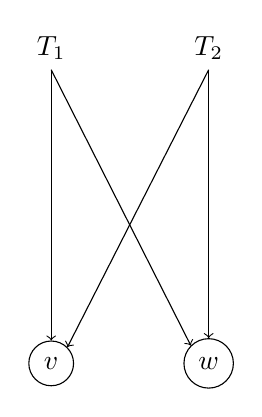
\begin{tikzpicture}
      \node (t1) at (-1,0) {$T_1$};
      \node (t2) at (1,0)  {$T_2$};
      \node (v) [draw,shape=circle] at (-1,-4) {$v$};
      \node (w) [draw,shape=circle] at (1,-4)  {$w$};

      \draw [->] (t1.south) -- (v.north);
      \draw [->] (t1.south) -- (w.north west);
      \draw [->] (t2.south) -- (v.north east);
      \draw [->] (t2.south) -- (w.north);
    \end{tikzpicture}
    \caption{Sequential Consistency}
  \end{subfigure}
  \begin{subfigure}[t]{0.3\textwidth}
    \centering
    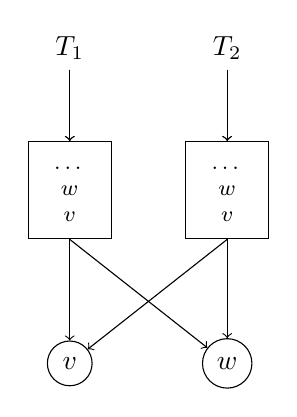
\begin{tikzpicture}
      \node (t1) at (-1,0) {$T_1$};
      \node (t2) at (1,0)  {$T_2$};
      \node (v) [draw,shape=circle] at (-1,-4) {$v$};
      \node (w) [draw,shape=circle] at (1,-4)  {$w$};

      \node (bt1) [draw] at (-1,-1.8) {\footnotesize\begin{tabular}{c} \ldots \\\midrule $w$ \\\midrule $v$ \end{tabular}};
      \node (bt2) [draw] at (1,-1.8) {\footnotesize\begin{tabular}{c} \ldots \\\midrule $w$ \\\midrule $v$ \end{tabular}};

      \draw [->] (t1) -- (bt1);
      \draw [->] (t1) -- (bt1);
      \draw [->] (t2) -- (bt2);
      \draw [->] (t2) -- (bt2);

      \draw [->] (bt1.south) -- (v);
      \draw [->] (bt1.south) -- (w);
      \draw [->] (bt2.south) -- (v);
      \draw [->] (bt2.south) -- (w);
    \end{tikzpicture}
    \caption{Total Store Order}
  \end{subfigure}
  \begin{subfigure}[t]{0.3\textwidth}
    \centering
    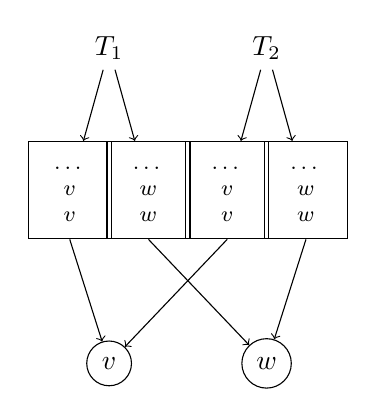
\begin{tikzpicture}
      \node (t1) at (-1,0) {$T_1$};
      \node (t2) at (1,0)  {$T_2$};
      \node (v) [draw,shape=circle] at (-1,-4) {$v$};
      \node (w) [draw,shape=circle] at (1,-4)  {$w$};

      \node (bt1v) [draw] at (-1.5,-1.8) {\footnotesize\begin{tabular}{c} \ldots \\\midrule $v$ \\\midrule $v$ \end{tabular}};
      \node (bt1w) [draw] at (-0.5,-1.8) {\footnotesize\begin{tabular}{c} \ldots \\\midrule $w$ \\\midrule $w$ \end{tabular}};
      \node (bt2v) [draw] at (0.5,-1.8) {\footnotesize\begin{tabular}{c} \ldots \\\midrule $v$ \\\midrule $v$ \end{tabular}};
      \node (bt2w) [draw] at (1.5,-1.8) {\footnotesize\begin{tabular}{c} \ldots \\\midrule $w$ \\\midrule $w$ \end{tabular}};

      \draw [->] (t1) -- (bt1v);
      \draw [->] (t1) -- (bt1w);
      \draw [->] (t2) -- (bt2v);
      \draw [->] (t2) -- (bt2w);

      \draw [->] (bt1v.south) -- (v);
      \draw [->] (bt1w.south) -- (w);
      \draw [->] (bt2v.south) -- (v);
      \draw [->] (bt2w.south) -- (w);
    \end{tikzpicture}
    \caption{Partial Store Order}
  \end{subfigure}
  \caption{Write buffering for two threads and two \texttt{CRef}s.}
  \label{fig:wb}
\end{figure}

We divide concurrency operations into three categories: \emph{synchronised}
operations impose a \emph{memory barrier}, which commits all buffered writes;
\emph{partially synchronised} operations commit one or more buffered writes to
the same \verb|CRef|; and \emph{unsynchronised} operations never cause a commit.

\paragraph{Phantom Threads}
In a sequentially consistent memory model, the set of runnable threads is
exactly the set of threads created by forking which are not blocked.  Under
relaxed memory, however, this is not the case.  For each write buffer, we
introduce one \emph{phantom thread}.  When scheduled, a phantom thread will
commit the oldest write in its corresponding buffer.

This may seem like an odd approach: why create new threads to model relaxed
memory?  The advantage is that systematic concurrency testing techniques assume
there is only one source of nondeterminism: the scheduler.  If a second source
is added, such as when writes are committed, it is difficult to integrate this
with existing algorithms.  By using phantom threads, the two sources of
nondeterminism are unified, and existing algorithms just work.  We take this
approach from \cite{zhang2015}.

\section{Testing Concurrent Programs}
\label{sec:dejafu-testing}

\blindtext

\section{Soundness and Completeness}
\label{sec:dejafu-correctness}

\blindtext

\section{Case Studies}
\label{sec:dejafu-casestudies}

\blindtext

\subsection{The auto-update Package}
\subsection{Search Party}
\subsection{The Par Monad}

\section{\dejafu{} in the Wild}
\label{sec:dejafu-evaluation}

\blindtext

\subsection{Richness of the Abstraction}
\subsection{Porting Code}
\subsection{Integration with Existing Tools}

\section{Conclusions and Future Work}
\label{sec:dejafu-conclusions}

\blindtext
